\section{Introduction}

As a global public health issue resulting in extreme societal, economic, and political disruption, the COVID-19 pandemic has highlighted the importance of proactive epidemic forecasting, critical in providing response guidance for policymakers and healthcare authorities. However, the latency problem commonly exists in public health surveillance data streams. It often causes imperfect or even error-prone situational awareness \cite{McGough2020}\cite{Rosenfeld2021} and brings challenges to real-time forecasting accuracy. 

To be more detailed, the latency problem refers to the situation where the observations or statistics provided by the surveillance systems are most up-to-date but not finalized. The initially released data is usually revised/corrected through a process known as the \textit{backfill} phenomenon. Except for errata, some data will only be reported once with some degree of reporting delay, which is regarded as a special case of backfill. The term \textit{backfill correction} we used throughout this paper refers to providing projection of finalized values based on the current observations.

Many factors can affect the magnitude of backfill, such as laboratory confirmation, infrastructure difficulties, coordination efficiency between health authorities and government\cite{reich2019collaborative}\cite{Chakraborty2018}, etc. Understanding the backfill pattern is crucial, as it could lead to intelligent strategies for making accurate projection of the observations that are far from finalized. Backfill has been commonly mentioned in public health studies, ranging from influenza\cite{chakraborty2018know}, dengue\cite{rangarajan2019forecasting} to COVID-19 forecasting\cite{rodriguez2021deepcovid}. Different approaches have been proposed to address the backfill problem retrospectively and in real time. One common strategy is to re-scale real-time reports by estimating scaling factors from historical data\cite{lawless1994adjustments}\cite{hohle2014bayesian}. Other ones such as backcasting handle the reporting error by generating past weeks’ validation data using the most recent data reports for those weeks and accounting for uncertainty in reporting patterns\cites{brooks2018nonmechanistic}. Nowcasting studies deal with backfill via complicated statistical or machine learning methods\cite{li2021bayesian}\cite{mjahja2021} strictly based on incomplete data. 

It is worth noting that backfill correction is more challenging for COVID-19 from two perspectives: 1) SARS-CoV-2 is constantly changing, and the dominant variant is continuously updated while the epidemic pattern of seasonal influenza is more stable and less noisy; 2) the degree of concern and response measures from the government and healthcare authorities to COVID-19 is constantly changing as well, making the pattern of data collation and revision difficult to predict. Despite this, digital surveillance, developed in the recent years especially during the COVID-19 pandemic, play an indispensable role in understanding and modeling backfill patterns. Data revision history is no longer ignored but well captured and archived with support of new technology and methods.


In this paper, we focus on making projection of the finalized values of observations in \textit{real-time} and measuring the uncertainty in projection, laying out a framework for an operational backfill correction system using provisional data. At any given date $s$, we are forced to use data that is guaranteed to be available at date $s$. Specifically, backfill correction takes as input all the revisions of observations with finalized values included as the target, and output the estimation of probability distribution over the target variable based on the most up-to-date observations. There are two categories of observations that we mainly care about: 1) counts; 2) fractions. Take COVID-19 insurance claims data as an example, counts can be the number of outpatient insurance claims that's made for COVID-19 patients while fractions can be the percentage of COVID outpatient insurance claims in terms of total outpatient insurance claims.

An outline for this paper is as follows. In Section 2, we provide preliminary information about notations and the problem setup. The details of the model are described in Section 3. Section 4 covers evaluation of the results and comparing the backfill correction results made in real-time to those without correction. In Section 5, we conclude with a discussion and describe a few directions for future work.


\begin{figure}
    \centering
    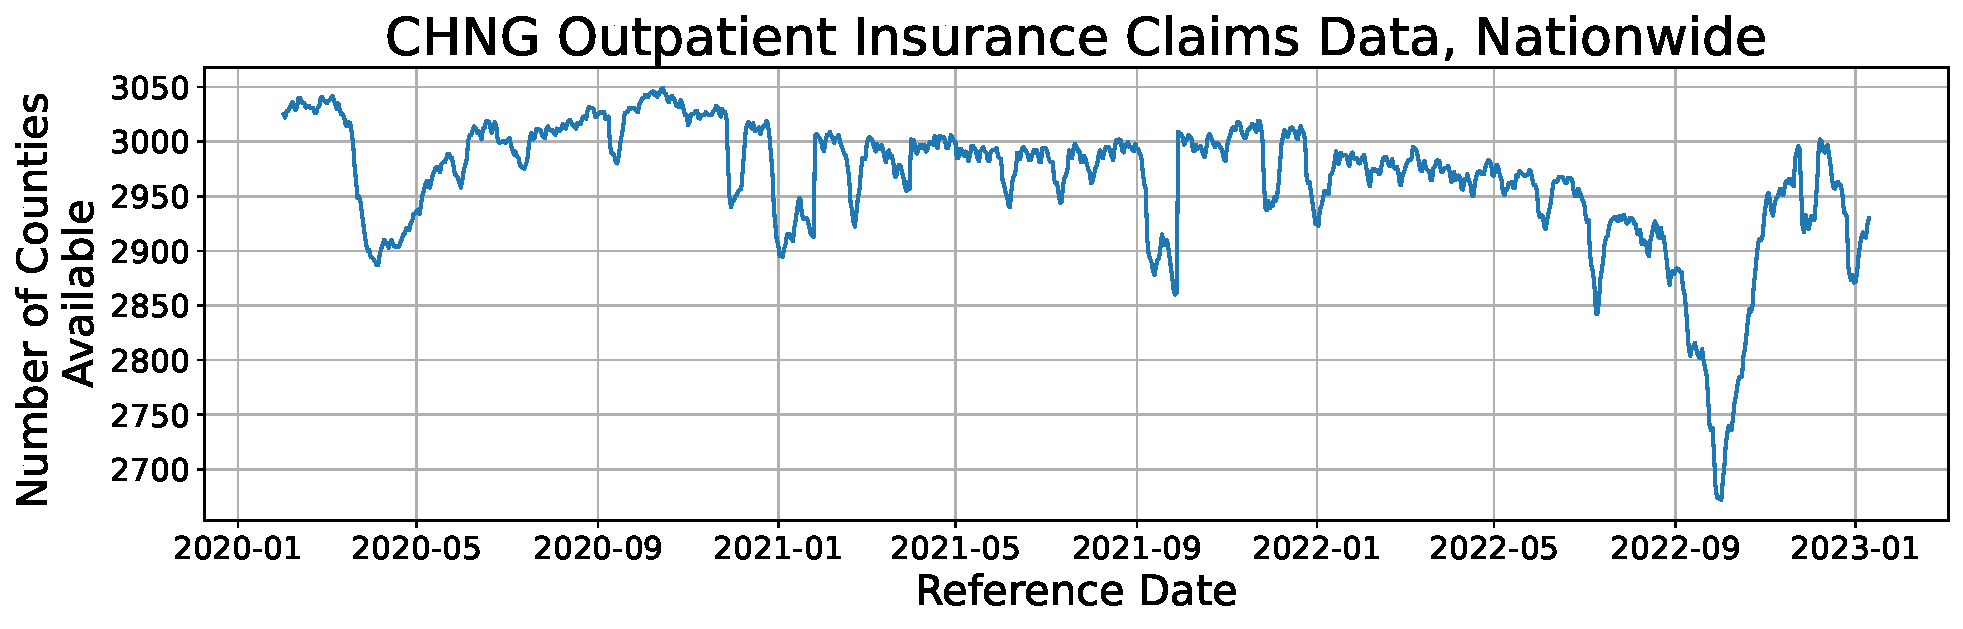
\includegraphics[width=\textwidth]{figs/available_counties.pdf}
    \caption{\textit{}}
\end{figure}